\section{Evaluation}
\label{sec:eval}
The setup in which our document modification approach operates is as
follows.  First, a ranking for a query is observed. Then, the approach
is applied to modify a given document so that the resulting document
will be ranked higher in the next induced ranking. In real dynamic
settings, other documents can change at the same time thereby
affecting the next ranking. Accordingly, we present online evaluation in a dynamic setting. In
addition, we present an offline evaluation intended to study specific
aspects of the approach.


\subsection{Experimental Setting}
\label{sec:expSet}
To perform online evaluation, we used our approach as a bot in
content-based ranking competitions which were inspired by
those of \citet{Raifer+al:17a} who analyzed publishing strategies.

In our competitions, which were approved by an international and an
institutional ethics committees, students in a course served as
documents' authors and were assigned to queries.  The students were
incentivized via bonuses to the course grades to write and modify
plain text documents of up to $150$ terms so that the documents will
be highly ranked for the queries. Students in the course could have attained
the maximal grade without participating in the competitions. The
students who participated signed consent forms and could have opted
out at any point in time.  Our bot received a document to be modified
so as to compete with the students for rank promotion. We organized a
competition for each of $15$ queries randomly sampled from the $31$
used by \citet{Raifer+al:17a}\footnote{Raifer et al.'s dataset is
  available at \url{https://github.com/asrcdataset/asrc}.}.  These
queries were originally selected from all topic titles for the Web
tracks of TRECs $2009$-$2012$ by the virtue of having a commercial
intent that can stir up ranking competitions\footnote{The topic IDs of
  the $15$ queries are: $3$, $10$, $18$, $32$, $33$, $34$, $48$, $51$,
  $69$, $167$, $177$, $180$, $182$, $193$, and $195$.}.

  Two students took part in each competition for a query. No two students competed against each other for more than
  one query, and no student competed for more than three queries.  The
  two students competing for a query were provided at the beginning of
  the competition with the same example of a document relevant to the
  TREC topic the query represents.  Some of these documents were
  adopted from the dataset in \citet{Raifer+al:17a}; others were
  created by the authors of this paper using a similar approach to
  that in \citet{Raifer+al:17a}. The students had no incentive to
  stick to these original documents. Hence, in contrast to our bot,
  they had more freedom in promoting their documents. Furthermore, all
  students had prior experience in participating in similar content-based ranking
  competitions for queries other than those they
  were assigned to in our competitions.

  In the first round of the competition, the students submitted their
  modified documents to the search engine. They were then shown a
  ranking induced over a set of $5$ documents: their two documents and
  additional three 
  \firstmention{\planted} documents which were
    %adopted
    randomly selected
    from the first round of
    %the competition in
    Raifer et al.'s competitions.
  The students were not aware of the
  fact that other documents might not be written by students actually
  competing with them. The identities of
  all documents' authors were anonymized. Throughout the competition,
  the students had access to all documents in rankings.
  The ranking function, described below, was not disclosed to the students.
  
  Having observed the induced ranking, the two students could then
  modify their documents to promote them in the next ranking, and
  submit them for the second round of the competition. The most
  highly ranked \planted document in the first round, which was not
  also the most highly ranked in the entire ranking, and which was
  marked by at least three annotators out of five in Raifer et al's
  competitions as of high quality, was provided
  as input ($\curDoc$) to our bot. Our approach modified the document
  and submitted it ($\newDoc$) to the second round.
  For the other two
  \planted documents, their second-round versions in Raifer et al.'s
  competition were submitted to our second round. As additional baseline, we use a {\em
  simulated} {\bf static bot}: it receives the same
document in the first round as our bot, and simply submits it to the second round with no
modifications. Comparison with the static bot allows to evaluate
the merit of using a dynamic bot which responds to ranking.

  Our approach was designed for a single shot modification. Hence, our
  main evaluation is based on the ranking induced in the second round
  of the competition with respect to that induced in the first round. Furthermore, we used crowdsourcing
  (via the Figure Eight platform\footnote{\url{https://www.figure-eight.com/}})
  to assign quality and relevance labels to all documents in the competition as in Raifer
  et al.'s competitions, using their annotation guidelines. Each document was annotated by five
  annotators. A document was deemed relevant or of high content quality if it was marked as such by at least three annotators. Although not designed for iterative document modification, we
  let our bot participate in two additional rounds modifying its document in response to rankings.
  %We did not bound the number of previous rankings the bot observes (i.e., the value of $p$ in Section \ref{sec:framework}).
%  The bot utilized in its rank-promotion features information about all rankings as from the first round to the current round. The students had access to the exact same information.


\myparagraph{Document ranking function}
Similarly to \citet{Raifer+al:17a}, we used the state-of-the-art LambdaMART learning-to-rank (LTR) method
\cite{Wu+al:10a} with $25$ standard content-based features as the search engine's ranking function. These features were either used in Microsoft's learning-to-rank datasets\footnote{\url{https://tinyurl.com/rmslr}}, or are query-independent document
quality measures \cite{Bendersky+al:11a}. Further details regarding the ranking method are provided in the appendix. 


%\subsubsection{Document ranking function}
%\label{sec:rankFunc}
%For document ranking, we used the same learning-to-rank approach, and features, used by Raifer et
%al. \cite{Raifer+al:17a} in their fundamental ranker. Specifically,
%the state-of-the-art LambdaMART learning-to-rank (LTR) approach
%\cite{Wu+al:10a}\footnote{We used the RankLib implementation: \url{www.lemurproject.org/ranklib.ph}.}  was used with $25$ content-based features. (Recall that
%we focus on content-based modifications.). These features were either
%used in Microsoft's learning-to-rank datasets\footnote{\url{https://tinyurl.com/rmslr}}, or are query-independent document
%quality measures --- specifically, stopword-based measures and the
%entropy of the term distribution in a document --- demonstrated to be
%effective for Web retrieval \cite{Bendersky+al:11b}.

%To train the ranking function, we used the ClueWeb09 Category B collection
%and its $200$ topic-title queries (TREC $2009$-$2012$). We used the query likelihood retrieval approach \cite{Song+Croft:99a} with Dirichlet
%smoothed document language models; the smoothing parameter was set to
%$1000$~\cite{Zhai+Lafferty:01a}. Documents assigned a score below $50$
%by Waterloo's spam classifier were removed from rankings. The resultant top-$1000$ documents were used for training. We used default
%values of the free parameters in the implementation except for the number of leaves and trees
%which were selected from $\set{5,10,25,50}$ and $\set{250,500}$,
%respectively, using five-fold cross validation performed over queries:
%five folds were used for training and one for validation of these two
%parameters; NDCG@5 was the optimization criterion. We select the
%parameter values that result in the best NDCG@5 over all $200$ queries
%when these were used as part of the validation folds.

 
\myparagraph{Ranking passage pairs}
\label{sec:offline}
Our document modification approach is based on learning-to-rank
passage pairs. Since the documents are short (up to $150$ terms), we
used sentences for passages. We trained the approach using the
rankings available for all $31$ queries from round $6$ of Raifer et al.'s competitions; RankSVM was the
passage-pair ranker~\cite{Joachims:06a}. Our training dataset contains $57$ documents which serve for $\curDoc$ with overall $3399$ passage
pairs $(\psgSrc,\psgTarget)$.

%For each document there are, on average,
%$59.6$ such pairs that are to be ranked.
%(with standard deviation of $42.32$) that are to be ranked.


Additional details about the choice of training data and training RankSVM
and Word2Vec --- used for some features --- are provided in
the appendix. We now describe the creation of rank-promotion ($\rankPromoteLabel$) and local-coherence maintenance ($\coherenceLabel$), henceforth coherence, labels for training.

%approach is based on learning-to-rank, for a given document $\curDoc$ which we want to rank-promote, passage pairs,
%$(\psgSrc,\psgTarget)$, where $\psgSrc$ is a passage in $\curDoc$, and $\psgTarget$ is a
%passage in a document among the most highly ranked in the current
%ranking, $\curRank$. (Refer back to Section \ref{sec:framework} for
%details.)  To train our approach, we used all $31$ queries and all the
%documents submitted for these queries in round $6$ of Raifer et al.'s
%competition \cite{Raifer+al:17a}\footnote{In round $5$ of Raifer et al.'s
%  competition, the incentive system has changed
%  \cite{Raifer+al:17a}. Hence, we selected a round which is after the
%  change.}, except for those which were not marked as of high quality
%by at least $3$ out of $5$ crowdsourcing annotators
%\cite{Raifer+al:17a}. To induce document ranking, we used the 
%ranking function from Section \ref{sec:rankFunc} which was also used in the online evaluation described
%above. Recall that our approach has no knowledge of the document ranking
%function. As the documents are quite short (as noted above, their
%length is at most $150$ terms), we use sentences as passages in our
%approach.

%We let our approach modify a document, $\curDoc$, which is either the
%lowest ranked or the second highest ranked 
%for a query. Thus, we have a mix of low ranked and high ranked
%documents which we let our approach train with. As a result, for each
%query, we consider two identical current rankings, $\curRank$, over
%the given documents. In each of these two rankings, a single document
%--- ranked second or last --- is designated as $\curDoc$. And, we
%induce two new rankings, $\nextRank$, where $\curDoc$ was modified by
%our approach to $\newDoc$. The rest of the documents are not modified;
%i.e., we train our approach by ``assuming'' that other documents do
%not change\footnote{The alternative would have been to have other
%  documents modified simultaneously to $\curDoc$. However, this would have introduced much noise
%  to the learning phase as the ranking of $\newDoc$ could have
%  changed with respect to that of $\curDoc$ not necessarily due to the modification of $\curDoc$, but rather
%  due to those of others.}. Our training dataset contains $57$ documents which serve for $\curDoc$ with overall $3399$ passage
%pairs $(\psgSrc,\psgTarget)$. For each document there are, on average,
%$59.6$ such pairs (with standard deviation of $42.32$) that are to be ranked.

%Some of the features on which our approach relies, namely
%{\simSrcPrevTopTF}, {\simTargetPrevTopTF}, {\simSrcPrevTopWtV} and
%{\simTargetPrevTopWtV}, utilize information about the past $p$
%rankings. Thus, as was the case above in the online evaluation, we let
%our approach observe all current and past rankings (i.e., $p=6$) where these were
%induced using our ranking function over the documents in each of the
%first five rounds of Raifer et al.'s competition \cite{Raifer+al:17a}.





%As noted in Section \ref{sec:framework}, any feature-based
%learning-to-rank approach can serve for our passage-pair ranking
%function. Since we do not have large amounts of training data, we used
%a linear RankSVM~\cite{Joachims:06a}\footnote{\url{https://www.cs.cornell.edu/people/tj/svm_light/svm_rank.html}};
%all free parameters were set to default values of the implementation,
%except for $C$ which was set using cross validation. Specifically, we
%used $5$ fold cross validation over all $57$ documents\footnote{Recall that ranking of passage pairs is performed with respect to a specific document $\curDoc$.} which serve as $\curDoc$, where $4$ folds were used to train RankSVM and% the one fold (validation) was used to
%set $C$'s value ($\in \set{0.001. 0.01, 0.1}$) by optimizing for
%NDCG@5. (More details about evaluation measures are provided below.) As each document is part of a single validation fold, we set $C$ to the value that optimized NDCG@5 over all documents when these were part of a validation fold. The trained approach was then used for the bot in the online evaluation --- i.e., ranking competitions.

%As described in Section \ref{sec:framework}, our approach utilizes, as
%features, Word2Vec-based similarities. We train a 
%query-based Word2Vec model \cite{Diaz+al:16a} using the {\rm gensim}
%package\footnote{https://radimrehurek.com/gensim/models/word2vec.html}. Specifically,
%for a query $\query$, the model was trained on the top-$10000$ documents
%retrieved from ClueWeb09 Category B for $\query$ using the query likelihood retrieval model
%\cite{Song+Croft:99a}; spam removal was not applied here. Default parameter values of the {\rm gensim}
%package were used, except for the threshold of number of occurrences per word which
%was set to $0$, the window size which was set to $8$, and the vector size which was set to $300$.  

%\myparagraph{Rank-promotion and coherence labels}
%Our approach is trained using rank-promotion
%($\rankPromoteLabel$) and local-coherence maintenance ($\coherenceLabel$) labels.

For each document $\curDoc$ in a
ranking $\curRank$ in the training set, we create, as described in Sect. \ref{sec:framework}, passage pairs
$(\psgSrc,\psgTarget)$ where $\psgSrc \in\curDoc$ and
$\psgTarget$ is any passage in documents highly ranked in $\curRank$. We replace $\psgSrc$ in $\curDoc$
with $\psgTarget$ to yield $\newDoc$, and induce a new ranking
$\nextRank$.
%\footnote{An underlying assumption is that we can submit
%  modified documents to a search engine and observe new rankings.}.
The rank-promotion label, $\rankPromoteLabel$, is $0$ if the rank
position of $\newDoc$ in $\nextRank$ is the same or worse than that of
$\curDoc$ in $\curRank$; otherwise, $\rankPromoteLabel$ is the
difference between $\newDoc$'s rank in
$\nextRank$ and $\curDoc$'s rank in $\curRank$. As there are $5$
documents in each ranking,
%the rank difference is bounded by 4, and
$\rankPromoteLabel$ is in $\set{0,4}$ as mentioned in
Sect. \ref{sec:framework}

%\footnote{All competitions but one in Raifer et al. \cite{Raifer+al:17a} were between $5$ students. There was a single query with $6$
%  competing students \cite{Raifer+al:17a}. The rank difference for
%  the document ranked sixth turned out to also be bound by $4$.}.

To produce a coherence label for
$(\psgSrc,\psgTarget)$, we aggregated the labels assigned by human
annotators in two different crowdsourcing tasks performed using
Amazon's Mechanical Turk.
%We used a pairwise preference approach which is known
%to be more effective for human annotations.
%Specifically, we create two different coherence labels
%for $\newDoc$ with a grade $\coherenceLabel_{basic}$ in $\set{0, 1,
%  \ldots 5}$ and use their arithmetic mean as the final coherence
%label, denoted $\coherenceLabel$.
In the first
%coherence
task,
%label was
%produced by showing
the annotators were shown both $\curDoc$ and $\newDoc$, where
$\psgSrc$ was highlighted in $\curDoc$ and $\psgTarget$ was highlighted
in $\newDoc$.
%Fiana: I'm removing this part as it seems unnecessary and and is a bit confusing.
%The annotators were told that one of the two documents is
%the original one.
%(which is coherent) whose highlighted passage was replaced with the
%highlighted passage in the second document.
%Then,
The annotators were asked to mark which of the two documents was the
original. The coherence label is the number of annotators,
among the $5$ assigned to the task, who failed identifying $\curDoc$
as the original.

The
second coherence label was produced by showing $\newDoc$ to annotators
and telling them that it was obtained by replacing a passage in a document they did not see. The annotators were asked to point to the passage which
presumably replaced a passage in that document; all passages in the document were marked. The number of annotators who did not
identify $\psgTarget$ as the replacing passage is the coherence label.

We scale the arithmetic mean of the two coherence labels by $\frac{4}{5}$ to have
the resultant coherence label, $\coherenceLabel$,
in $\set{0,1,\ldots,4}$ as for the rank-promotion
label. We then use the harmonic-mean approach described in Sect. \ref{sec:framework} to aggregate the coherence and rank-promotion labels. The resulting label, $l$, is a real number in $\set{0,4}$. To also induce binary labels, if the graded label $l$ is $ \ge 1$, then the binary label is $1$ and otherwise it is $0$.
%Hence, all labels of pairs, according to all three approaches
%just described, are real numbers in $\set{0,4}$. (Those for \rdc are integers in $\set{0,1,\ldots,4}$.) To induce binary labels, if the graded label is $ \ge1$, then the binary label is $1$ and otherwise it is $0$.

Since there was no a-priori reason to favor rank-promotion
over coherence and vice versa for {\em training} the bot for the
competitions, we have set $\beta=1$ in the harmonic-mean used to
aggregate coherence and rank-promotion graded labels. 

\myparagraph{Offline evaluation} We used the round-6 data from
\citet{Raifer+al:17a} to evaluate the rank-promotion and
local-coherence maintenance of our passage-pair ranker. The parameter $\beta$ that governs the harmonic mean used for label
aggregation (see Sect. \ref{sec:framework}) was set to values in
$\set{0,0.5,1,2,10^3,10^5,10^9}$. Each value entails a
different experimental setting as the labels change.
%\footnote{Hence, the RankSVM model is different for each value of $\beta$ and the setting is not that of multiple comparisons of the same hypothesis. Accordingly, correction (e.g., Bonferroni) for multiple hypothesis testing is not called for.} We train our approach with the same value of $\beta$ used for evaluation.

%$three aggregation
%$methods for the respective labels: \rdc, \arith and \harm. The same aggregation method was used for training RankSVM and for evaluation. \arith and \harm are dependent on a free parameter $\beta$, with values in $\set{0,0.1,\ldots,1}$ for \arith, and values in $\set{0,0.5,1,2}$ for \harm. Each value of $\beta$ for these two methods entails a different evalua$tion setting which we report.

Recall that
for document $\curDoc$, the highest ranked passage pair,
$(\psgSrc,\psgTarget)$, is used to produce $\newDoc$. To evaluate the
rankings over passage pairs for documents, we use MAP (over all
possible passage pairs per document), NDCG@1, NDCG@5, P@1 (precision
of the top pair) and TOP; TOP is either the rank promotion (in
terms of number of positions) of $\newDoc$ in $\nextRank$ with respect
to $\curDoc$ in $\curRank$ if it was indeed promoted or $0$ if it was not (or even demoted). In contrast to the other evaluation measures, TOP does not account for coherence; the NDCG measures use the graded
labels $l$ and the MAP and P@1 measures use the binary labels described
above. Details of the cross validation used are provided in the appendix.
%The passage-pair ranking is performed for each $\curDoc$
%separately. Here, we used five-fold cross validation over all $57$
%documents which serve as $\curDoc$, with three folds used for training
%RankSVM, one fold (validation) for setting its $C$ value using the value
%range specified above, and one fold for testing. The optimization
%criterion for the validation was NDCG@5. Each document is part of a
%single test fold. We report for each evaluation measure the average of
%its values for all these documents ($57$ overall) when they were part
%of a test fold.
As a baseline to our approach we use random
ranking, denoted \firstmention{\random}, over all passage pairs for
document $\curDoc$. We induce $10$ such random rankings and report the average performance over them. Statistically significant differences between our
approach and \random are determined using the two-tailed paired t-test with $p \le 0.05$.




%Note that none of the evaluation measures mentioned above,
%except for TOP, can be compared across the three approaches. We found
%that \harm yielded the highest TOP, as shown in Section
%\ref{sec:expResults}, and hence it was used to train the bot.



%\subsection{Experimental Results}
%\label{sec:expResults}
%In Section \ref{sec:onlineResults} we present the results of our online evaluation; that is, the analysis of the ranking competitions we organized in which our approach participated as a bot. In Section \ref{sec:offlineResults} we present the offline evaluation of our ranking method for passage pairs which is used for document modification in the bot. 



\subsection{Results of the Ranking Competitions}
\label{sec:onlineResults}
%We now turn to analyze the ranking competitions we organized.
%Recall
%from Sect. \ref{sec:expSet} that in the first round of a competition
%for a query, two students submit their documents, and in addition we
%use three {\bf planted} documents. One of these three planted documents is prov%ided
%to the bot which
%modifies it based on observing the
%first round ranking, and submits it to the second round. The two students also
%respond to the first round ranking and submit their (modified)
%documents for the second round. The remaining two planted documents
%(those not used by our bot) are replaced in the second round with
%their second-round versions from Raifer et al.'s competition which used the same queries and a similar ranker\footnote{If a document was the highest ranked in the first round in \cite{Raifer+al:17a}, we used the same document for the second round in our competition.}

%As additional reference comparison, we use a {\em
%  simulated} {\bf static bot}: it replaces our bot, receives the same
%document, and simply submits it to the second round with no
%modifications. Comparison with the static bot allows to evaluate
%the merit of using a dynamic bot which responds to ranking.

%To summarize, we have three players who actually participated in each
%competition for a query: two students participating in our competition and our
%bot. In addition, we have the two students from Raifer et al.'s
%competition whose documents we planted, thereby
%having five documents ranked for each query. The static bot is an
%additional simulated player that is considered as an alternative to our bot.

There are
five ``players'' per query in each competition round: two students from our competitions, two students
from Raifer et al.'s competitions whose documents were planted, and
the bot.

We analyzed the competitions using five evaluation measures.
The first three measures quantify ranking properties, and are computed
per player and her document for a query. The values for our students
and Raifer et al.'s are averaged over
the students. The averaged values, and the values for the bot and the static bot, are averaged over
queries. The first measure, {\bf average rank}, is 
the rank of the player's document, averaged as described
above; the highest rank is $1$. The {\bf raw promotion} and {\bf
  scaled promotion} measures quantify the change of a document's rank between rounds $1$ and $2$. The documents at rank $1$ are not considered as they can only be demoted. Raw promotion is the number of
positions by which the document was promoted (demoted).
%the reported
%number is the summation of all per-query values for documents of the
%player.
The scaled promotion is the raw
promotion normalized by the maximum potential for promotion/demotion with respect to the
document's position.

%also considers the
%maximum potential for promotion or demotion with respect to the
%document's position. That is, the  are normalized with respect to this potential.

%The per-document values assigned by these three {\em ranking-based} evaluation measures are averaged over the documents of the player for the
%different queries.

The {\bf quality} scores are assigned by crowdsourcing
annotators (in our and in Raifer et al.'s competitions) and
attest to the quality of the document content. A document receives a
quality score of $1$ if at least three out of five annotators marked
it as of high content quality and a quality score of $0$,
otherwise. Using the same approach, we assigned documents with a
$0$/$1$ {\bf relevance} grades with respect to the TREC topic
represented by the query. For the quality and relevance measures, we use the ratio of quality (relevant) documents across queries,
and normalize with respect to the number of players where needed.

\begin{table}[t]
  \caption{\label{tab:main} Main result table. The best result in a block for each round is boldfaced. Promotion is with respect to the previous round, and hence, there are no promotion numbers for the first round. }
    \small
  %  \begin{tabular}{@{}llcc@{}}
\toprule
& & round 1 & round 2 \\ \midrule
  \multirow{4}{*}{average rank} & students & $3.200$ & $\;\:3.400$\\
%  & students-top & $ 2.200$ &  $2.266$ \\
  & \planted & $\mathbf{2.733}$ & $\;\:2.766$\\
  & static bot & $3.133$ & $\;\:3.399$ \\ 
  & our bot & $3.133$ & $\mathbf{\;\:2.667}$\\ \midrule
  \multirow{4}{*}{raw promotion} & students & NA & $-6$\\
%  & students-top & NA & $2$\\
  & \planted & NA & $-1$ \\
  & static bot & NA & $-4$  \\
  & bot & NA & $\mathbf{\;\:7}$ \\ \midrule
  \multirow{4}{*}{scaled promotion} & students & NA & $-0.136$ \\
 % & students-top & NA & $0.141$ \\
  & \planted  & NA & $-0.002$\\
  & static bot & NA & $-0.177$ \\
  & our bot & NA & $\mathbf{\;\:0.122}$ \\ \midrule
  \multirow{4}{*}{quality} & students & $0.867$ & $\;\:0.900$\\
%    & students-top & $0.865$ & $0.900$\\
  & \planted  & $0.400$ & $\;\:0.766$ \\
  & static bot & $1.000$ & $\mathbf{\;\:1.000}$  \\
  & our bot & $1.000$ & $\;\:0.933$\\ \midrule
    \multirow{4}{*}{relevance} & students & $0.933$ & $\;\:0.866$ \\
%    &  students-top & $0.866$ & $0.866$ \\
  & \planted  & $0.900$ & $\mathbf{\;\:0.966}$ \\
  & static bot & $0.866$  &  $\;\:0.866$ \\
  & our bot & $0.866$ & $\;\:0.866$ \\ \bottomrule
\end{tabular}

  \center
  \begin{tabular}{@{}llcc@{}}
\toprule
& & round 1 & round 2 \\ \midrule
  \multirow{4}{*}{average rank} & students & $3.200$ & $\;\:3.400$\\
%  & students-top & $ 2.200$ &  $2.266$ \\
  & \planted & $\mathbf{2.733}$ & $\;\:2.766$\\
  & static bot & $3.133$ & $\;\:3.399$ \\ 
  & our bot & $3.133 $ & $\mathbf{\;\:2.667 }$\\ \midrule
  \multirow{4}{*}{raw promotion} & students & NA & $-0.200$\\
%  & students-top & NA & $-0.200$\\
  & \planted & NA & $0.000$ \\
  & static bot & NA & $-0.266$  \\
  & our bot & NA & $\mathbf{\;\:0.466 }$ \\ \midrule
  \multirow{4}{*}{scaled promotion} & students & NA & $-0.136$ \\
 % & students-top & NA & $0.141$ \\
  & \planted  & NA & $-0.002$\\
  & static bot & NA & $-0.177$ \\
  & our bot & NA & $\mathbf{\;\:0.122 }$ \\ \midrule
  \multirow{4}{*}{quality} & students & $0.867$ & $\;\:0.900$\\
%    & students-top & $0.865$ & $0.900$\\
  & \planted  & $0.400$ & $\;\:0.766$ \\
  & static bot & $1.000$ & $\mathbf{\;\:1.000}$  \\
  & our bot & $1.000 $ & $\;\:0.933 $\\ \midrule
    \multirow{4}{*}{relevance} & students & $0.933$ & $\;\:0.866$ \\
%    &  students-top & $0.866$ & $0.866$ \\
  & \planted  & $0.900$ & $\mathbf{\;\:0.966}$ \\
  & static bot & $0.866$  &  $\;\:0.866$ \\
  & our bot & $0.866 $ & $\;\:0.866 $ \\ \bottomrule
\end{tabular}

% \begin{tabular}{@{}llcc@{}}
\toprule
& & round 1 & round 2 \\ \midrule
  \multirow{4}{*}{average rank} & students & $3.200$ & $\;\:3.400$\\
%  & students-top & $ 2.200$ &  $2.266$ \\
  & \planted & $\mathbf{2.733}$ & $\;\:2.766$\\
  & static bot & $3.133$ & $\;\:3.399$ \\ 
  & our bot & $3.133 (0.533)$ & $\mathbf{\;\:2.667 (0.400)}$\\ \midrule
  \multirow{4}{*}{raw promotion} & students & NA & $-0.200$\\
%  & students-top & NA & $-0.200$\\
  & \planted & NA & $0.000$ \\
  & static bot & NA & $-0.266$  \\
  & bot & NA & $\mathbf{\;\:0.466 (0.400)}$ \\ \midrule
  \multirow{4}{*}{scaled promotion} & students & NA & $-0.136$ \\
 % & students-top & NA & $0.141$ \\
  & \planted  & NA & $-0.002$\\
  & static bot & NA & $-0.177$ \\
  & our bot & NA & $\mathbf{\;\:0.122 (0.462)}$ \\ \midrule
  \multirow{4}{*}{quality} & students & $0.867$ & $\;\:0.900$\\
%    & students-top & $0.865$ & $0.900$\\
  & \planted  & $0.400$ & $\;\:0.766$ \\
  & static bot & $1.000$ & $\mathbf{\;\:1.000}$  \\
  & our bot & $1.000 (0.200)$ & $\;\:0.933 (0.133)$\\ \midrule
    \multirow{4}{*}{relevance} & students & $0.933$ & $\;\:0.866$ \\
%    &  students-top & $0.866$ & $0.866$ \\
  & \planted  & $0.900$ & $\mathbf{\;\:0.966}$ \\
  & static bot & $0.866$  &  $\;\:0.866$ \\
  & our bot & $0.866 (0.066)$ & $\;\:0.866 (0.200)$ \\ \bottomrule
\end{tabular}

%  \begin{tabular}{@{}llcc@{}}
\toprule
& & round 1 & round 2 \\ \midrule
  \multirow{4}{*}{average rank} & students & $3.200$ & $\;\:3.400$\\
%  & students-top & $ 2.200$ &  $2.266$ \\
  & \planted & $\mathbf{2.733}$ & $\;\:2.766$\\
  & static bot & $3.133$ & $\;\:3.399$ \\ 
  & our bot & $3.133 (0.533)$ & $\mathbf{\;\:2.667 (0.400)}$\\ \midrule
  \multirow{4}{*}{raw promotion} & students & NA & $-0.200$\\
%  & students-top & NA & $-0.200$\\
  & \planted & NA & $0.000$ \\
  & static bot & NA & $-0.266$  \\
  & bot & NA & $\mathbf{\;\:0.466 (0.400)}$ \\ \midrule
  \multirow{4}{*}{scaled promotion} & students & NA & $-0.136$ \\
 % & students-top & NA & $0.141$ \\
  & \planted  & NA & $-0.002$\\
  & static bot & NA & $-0.177$ \\
  & our bot & NA & $\mathbf{\;\:0.122 (0.462)}$ \\ \midrule
  \multirow{4}{*}{quality} & students & $0.867$ & $\;\:0.900$\\
%    & students-top & $0.865$ & $0.900$\\
  & \planted  & $0.400$ & $\;\:0.766$ \\
  & static bot & $1.000$ & $\mathbf{\;\:1.000}$  \\
  & our bot & $1.000 (0.200)$ & $\;\:0.933 (0.133)$\\ \midrule
    \multirow{4}{*}{relevance} & students & $0.933$ & $\;\:0.866$ \\
%    &  students-top & $0.866$ & $0.866$ \\
  & \planted  & $0.900$ & $\mathbf{\;\:0.966}$ \\
  & static bot & $0.866$  &  $\;\:0.866$ \\
  & our bot & $0.866 (0.066)$ & $\;\:0.866 (0.200)$ \\ \bottomrule
\end{tabular}

  \end{table}
\myparagraph{Main results}
Table \ref{tab:main} presents our main results. Recall that the document
the bot (and the static bot) received per query in the first round was of high quality. The static bot did not change the document for the second round in contrast to our bot.

We see in Table \ref{tab:main} that by all three ranking-based 
evaluation measures, our bot outperformed the two active students in our competitions (``students''), the two students from Raifer et al.'s competitions (``planted'') and the static bot. It is the only player who
has positive raw and scaled promotion values in the second round. Furthermore, 
the bot's documents started from an average rank slightly better than
that of the active students' documents ($3.133$ vs.  $3.2$), and after the modifications for the second round, they were
promoted to a higher average rank ($2.667$ vs $3.4$). The documents the bot received in the first round were ranked higher than, or the same as,  those of the active students for $53\%$ of the queries. The percentage increased to $67\%$ in the second round after the documents were modified by the bot and the students.

Comparison of our bot with the static bot in terms of average rank and
(scaled) rank promotion attests to the importance of a ``live''
bot which responds to rankings. We also see that the average quality of the documents of our bot in the second round ($0.933$) is higher
than that of the documents of the two students from our
competitions ($0.9$) and from Raifer et al.'s competitions ($0.766$).

Table \ref{tab:main} also shows that the document our bot
received in round $1$ from Raifer et al.'s competitions was not always
relevant. The bot did not hurt relevance, on average, by its modifications (second round). This is in contrast to the two active students whose documents in the second round
were, on average, less relevant than in the first.





\newcommand{\figWidth}{4.25cm}
\newcommand{\figHeight}{4cm}
\begin{figure*}[t]
\hspace*{-0.5cm}
  \begin{tabular}{cccc}
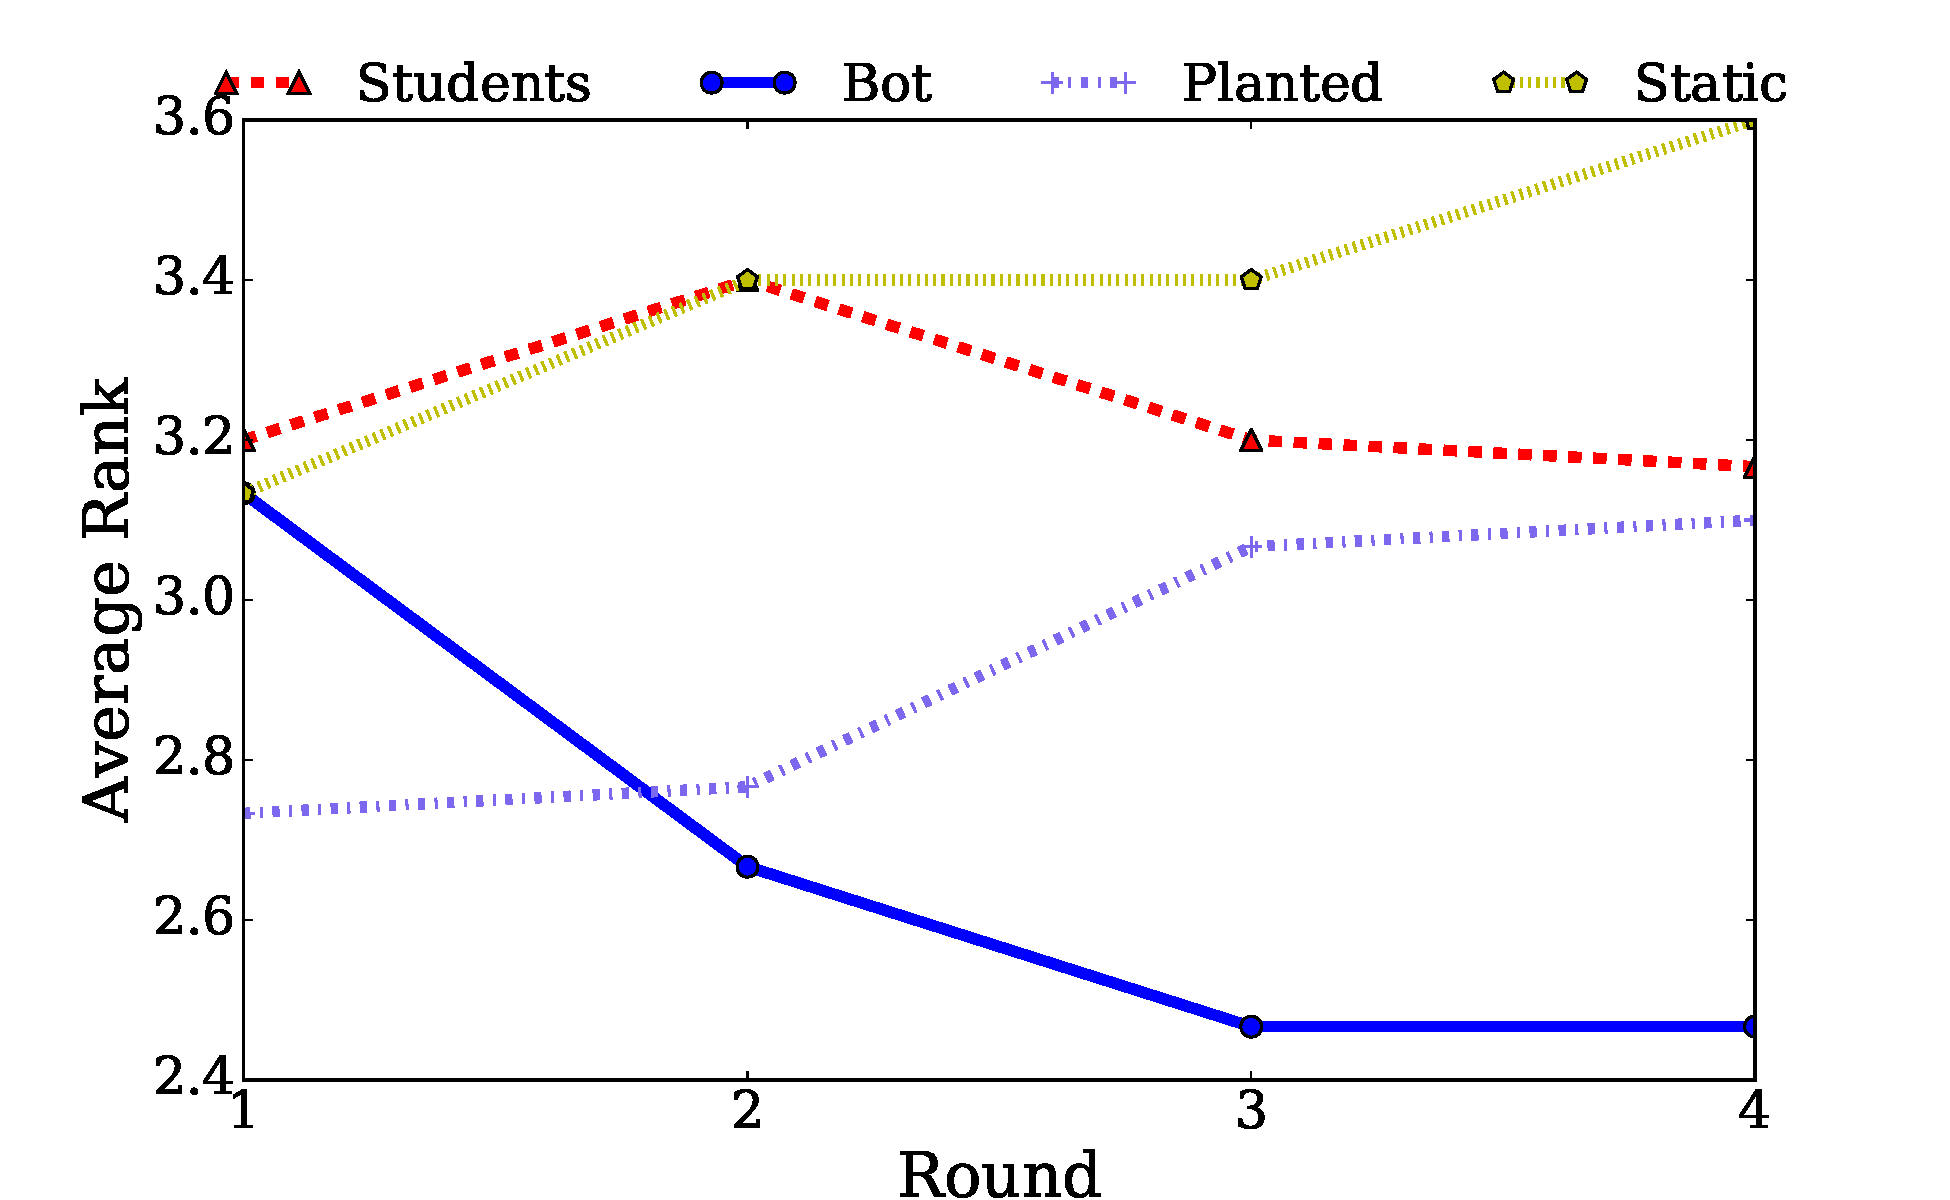
\includegraphics[width=\figWidth, height=\figHeight]{Results/average.pdf} &
\hspace*{-.5cm}        {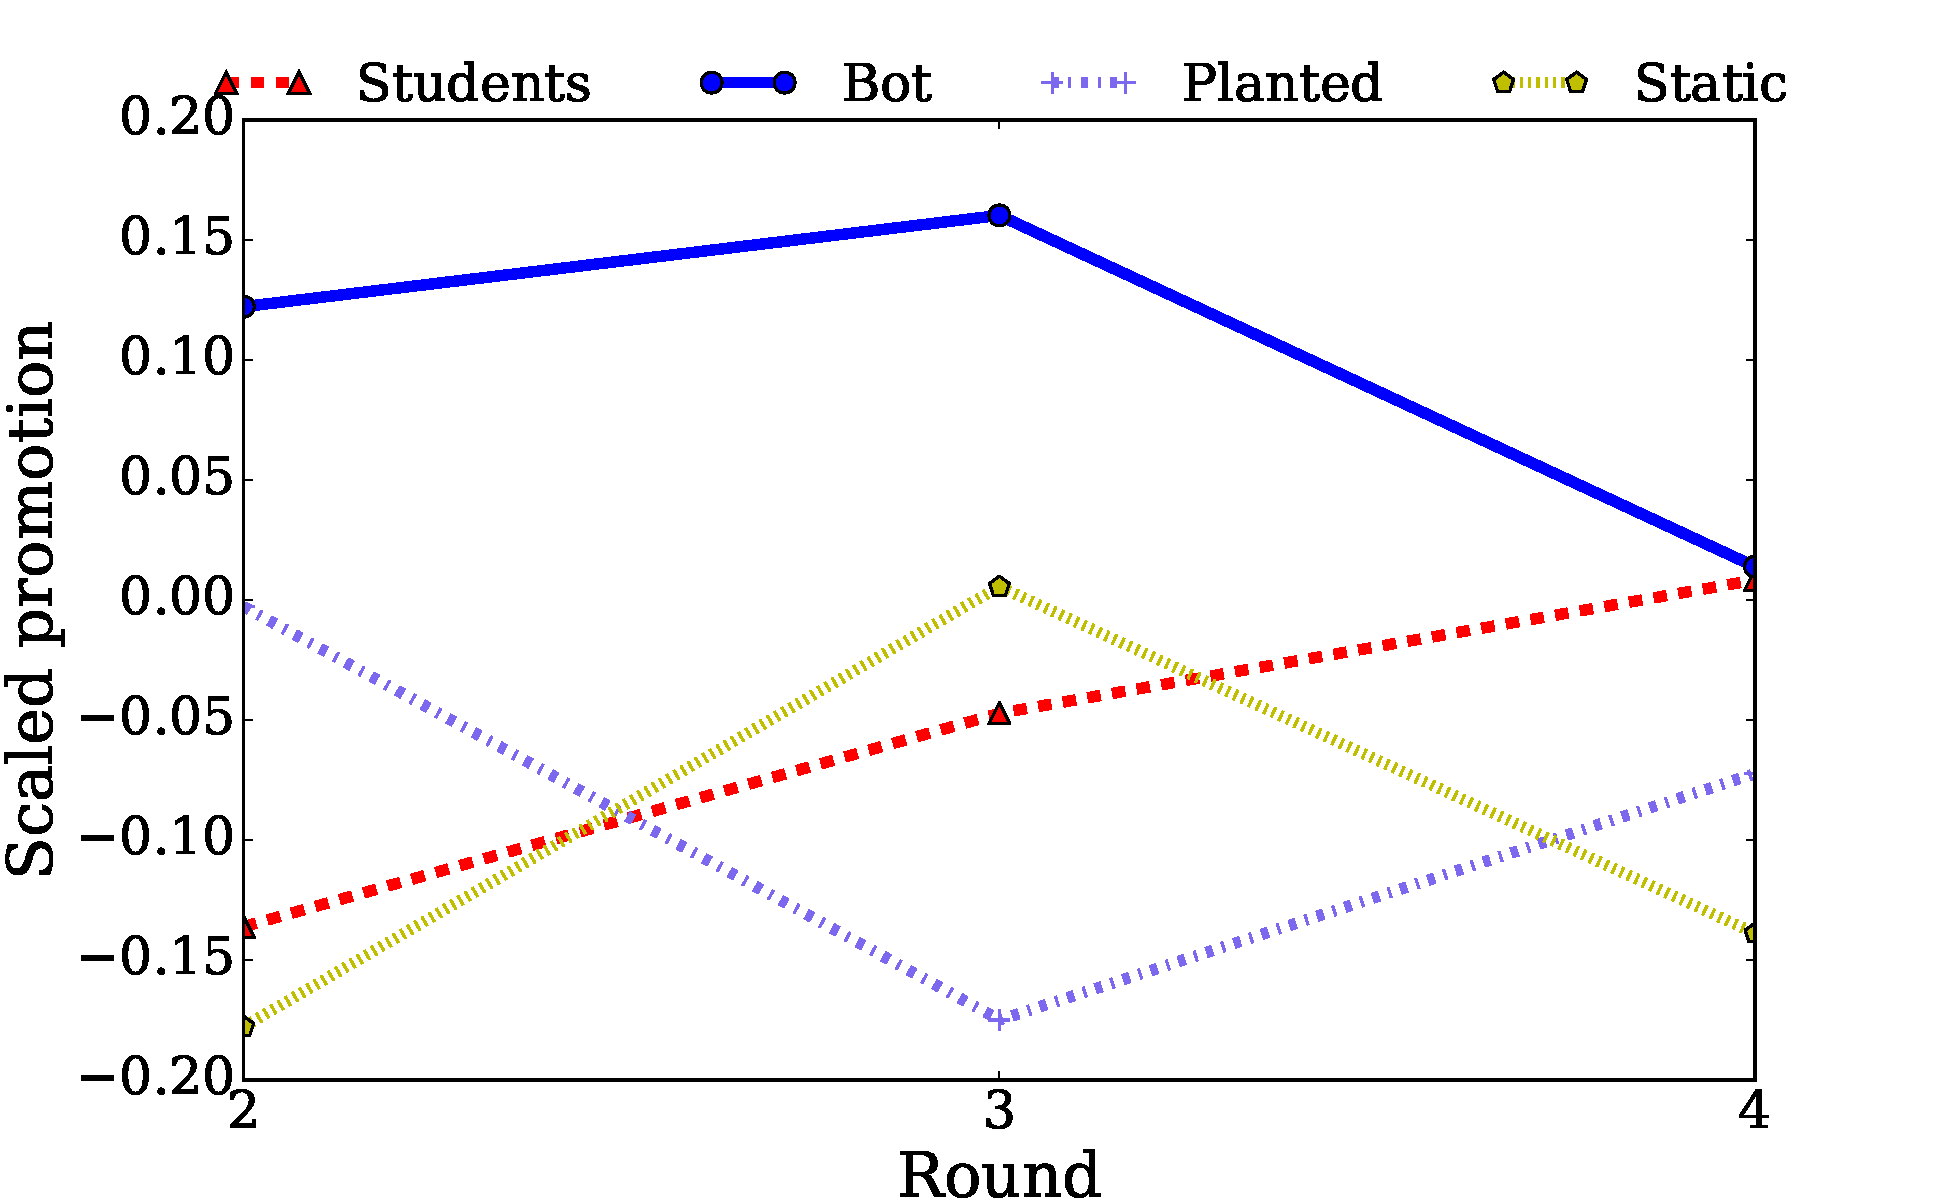
\includegraphics[width=\figWidth, height=\figHeight]{Results/potential}} &
 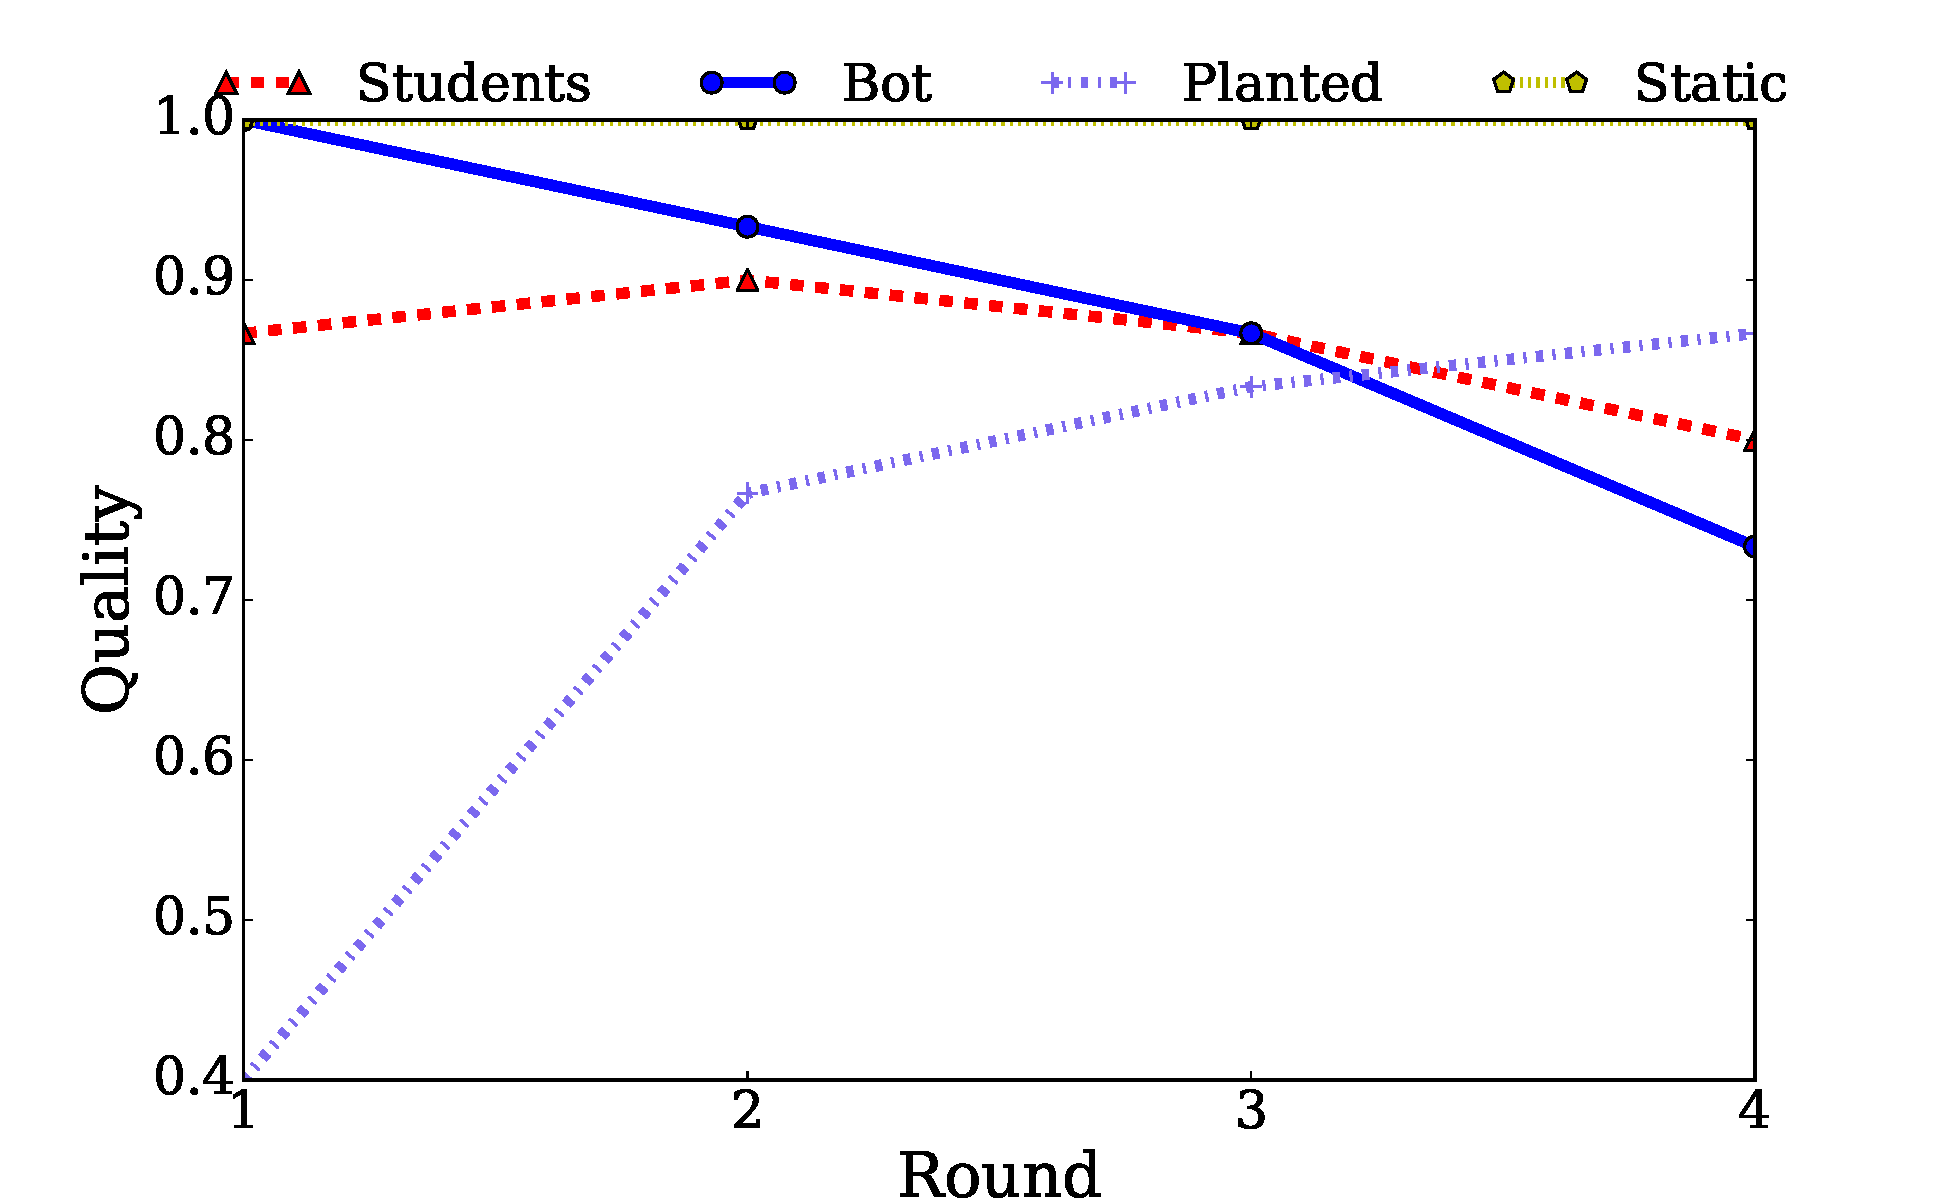
\includegraphics[width=\figWidth, height=\figHeight]{Results/ks} & 
\hspace*{-.5cm} 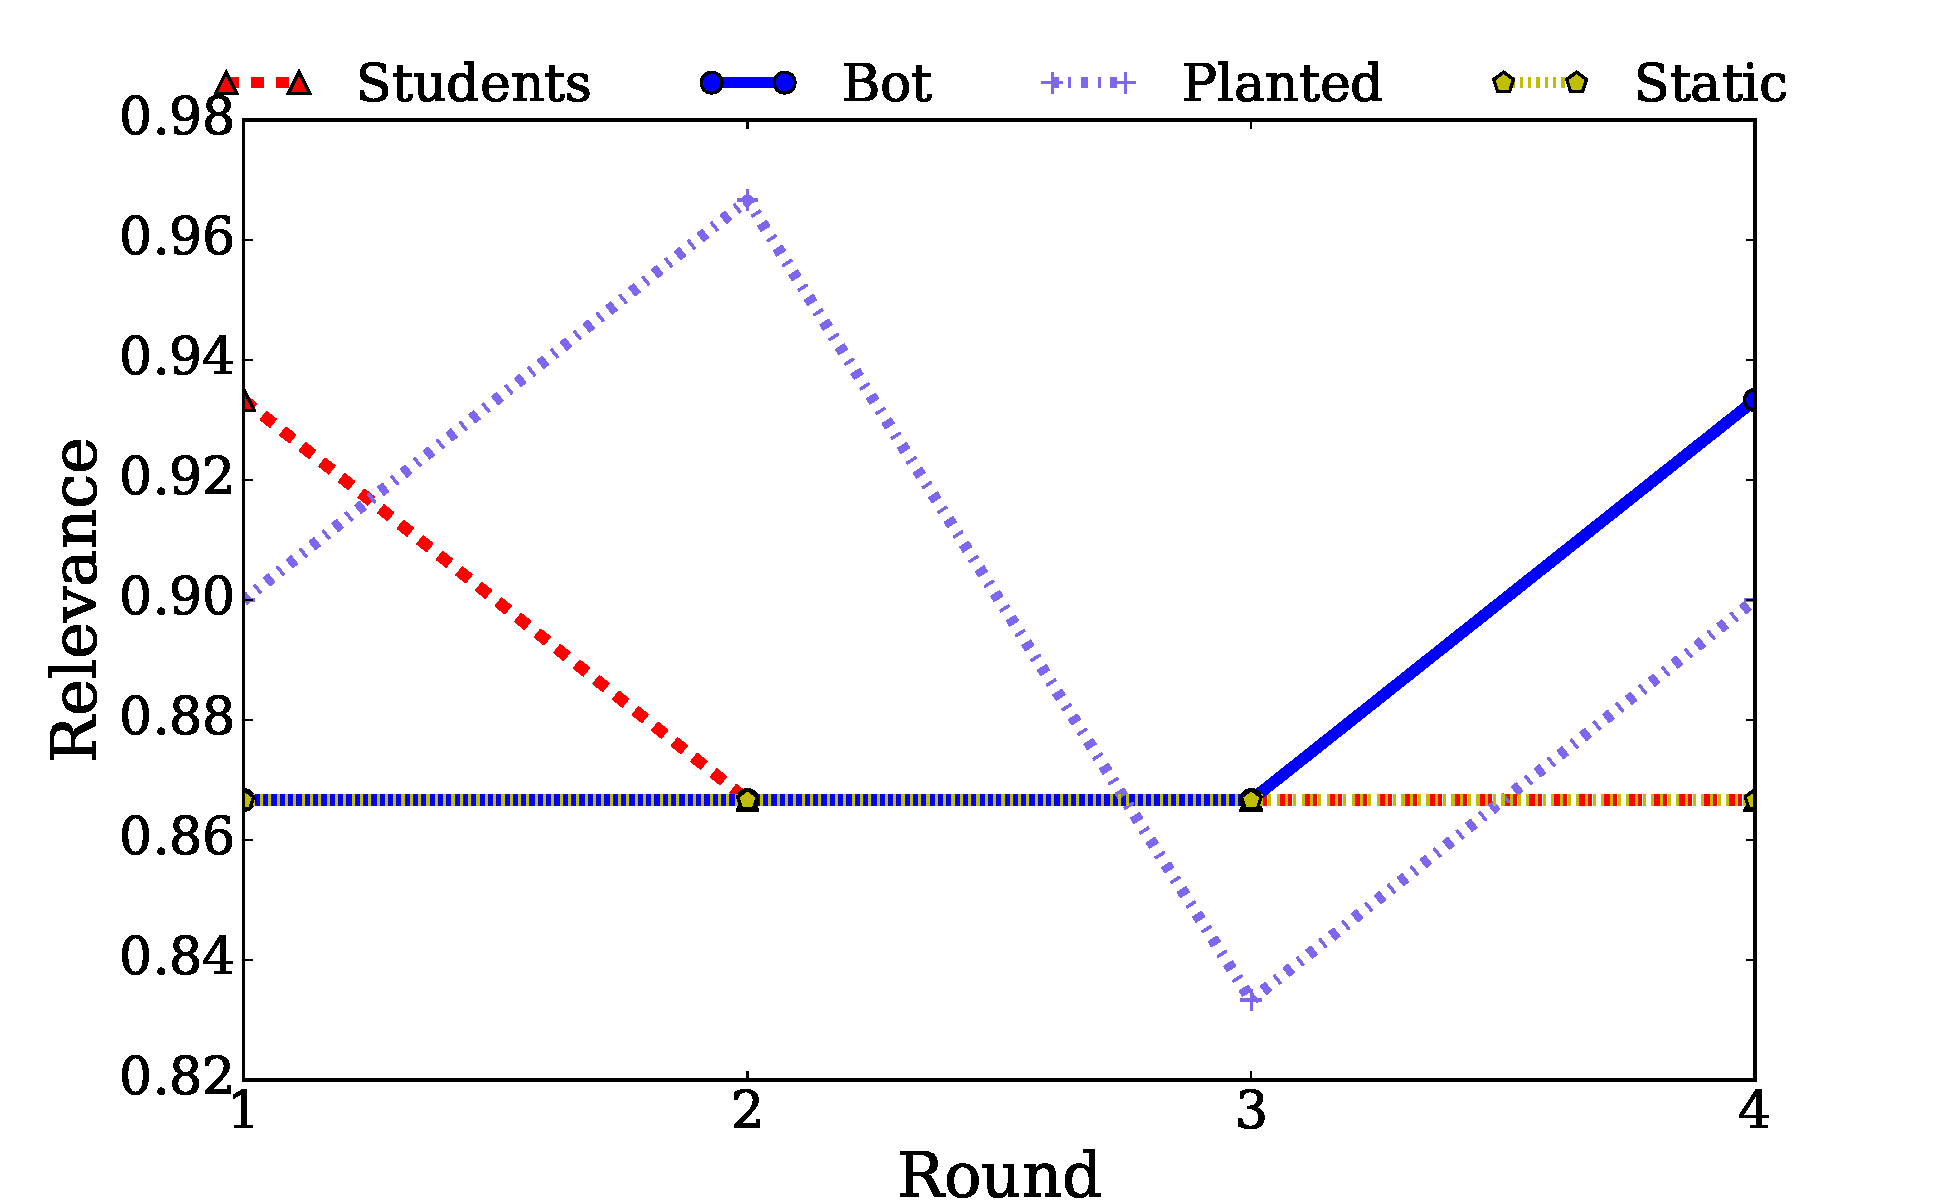
\includegraphics[width=\figWidth, height=\figHeight]{Results/rel} \\
  \end{tabular}
  \caption{\label{fig:competition} Analysis of the four rounds of the
    competition. The curves for the quality and relevance of the
    static bot are horizontal lines with values of $1$ and $0.867$, respectively.}
  \end{figure*}


The competitions' results are encouraging. The bot won
over the active students in terms of rank-promotion and content quality, and did not hurt relevance in contrast to the students. While the students had prior experience in ranking
competitions, the bot learned from a past static snapshot of a competition. (See Sect. \ref{sec:expSet}.)
Moreover, the students could have modified their documents in round $2$ without maintaining faithfulness to their documents from round $1$. This was not the case for the bot by design.

%which maintains faithfulness by the virtue of replacing a single sentence and the features it is trained with for maintaining coherence.


\subsubsection{Repeated Competitions}
Our bot was designed for a single shot (modification) response to a ranking. Yet, we let the competitions run for additional two
rounds with the bot and the two participating students.
%Specifically, (i) the bot
%modified the document it submitted for round $i$ ($\in \set{2,3}$),
%based on the induced ranking in this round, and submitted the
%resultant document to round $i+1$; (ii)
The two planted documents from
round $i$ ($\in \set{2,3}$) were replaced with their round $i+1$
versions from Raifer et al.'s competition.
%and
%(iii) the two students participating in the competition observed the
%ranking induced in round $i$ ($\in \set{2,3}$) and submitted their
%(modified) documents to round $i+1$.
%For a post-hoc analysis of the
%competition throughout the rounds, we analyzed,as at the above, the changes to %rankings
%if our bot was replaced
We also use as a baseline the static bot which did not change the
document our bot received in round $1$.
%The static bot did not participate in the competition as was the case above.

We see in Figure \ref{fig:competition} that
in terms of average rank, the bot wins over all other
players and the static bot. Furthermore, the bot is the only player whose scaled-promotion values are
always non-negative\footnote{The trends for raw promotion are similar. The results are omitted due to space considerations.}. These findings attests to the merits of the bot
in terms of rank promotion.

Figure \ref{fig:competition} also shows that the quality of the
bot's documents monotonically decreases. This is not a surprise as the
bot was designed for a single modification rather than a chain of
modifications; e.g., we did not prevent duplicate sentences in the modified documents, which the annotators penalized in terms of
quality. Yet, we note that even in round $3$, $85\%$ of the documents
produced by the bot were considered of high content quality
by the annotators.  A similar, although less steep, drop of quality is
observed as from round $2$ for the documents produced by the students
who participated in the competition. The increasing quality for the
planted documents can be attributed to the fact that in Raifer et
al.'s competitions, there were heavy ranking-penalties for producing
low-quality documents \cite{Raifer+al:17a}, which we did not impose in
our competitions.

Finally, we see in Figure \ref{fig:competition} that the bot did not
hurt the relevance of the documents it modified. In contrast, the documents produced by the students
who participated in our competitions were of lower relevance in round 2 than in round 1.

%(specifically, the move from
%round $1$ to round $2$), and those from Raifer et al.'s competition
%(the planted documents).

%\subsubsection{Document mimicking}
%Our approach for document modification was based on Raifer et al.'s
%\cite{Raifer+al:17a} theoretical and empirical finding with regard to
%the effectiveness of the following document promotion strategy: making
%a document become more similar to those most highly ranked in the past
%for the query of interest. As noted in Sect. \ref{sec:framework},
%the simple rational behind this strategy is that induced rankings are
%the only signal about the ranking function; thus, having a document
%become more similar to that highly ranked for the query potentially
%results in increased retrieval score. Indeed, in our approach, a short
%passage in a document is replaced with some passage of a  more
%highly ranked document for the same query. More specifically, our bot uses for
%round $i$ a passage $\psgTarget$ of a document more highly ranked than hers ($\curDoc$) in round $i-1$ to
%modify $\curDoc$ by replacing one of its passages ($\psgSrc$).

%In Figure \ref{fig:simWinner} we analyze this phenomenon of ``document
%mimicking''. We present the average cosine similarity of the TF.IDF vectors at round $i$ representing the documents produced by students participating in our competition, the planted documents and the document of our bot, with the  TF.IDF vector of the document most highly ranked in the previous round ($i-1$); self similarities are excluded.\footnote{For example, if the document of our bot was ranked first, it was not changed for the next round of the competition. Similarly, students did not tend to change their documents if they were ranked first.}
%We indeed see the increasing similarity patterns for both the students participating in the competition and for the bot, where the increase for the latter is much more steep. The similarity of the planted documents naturally decreases as these are documents from a different competition which were modified in response to different rankings.

%\begin{figure}[t]
%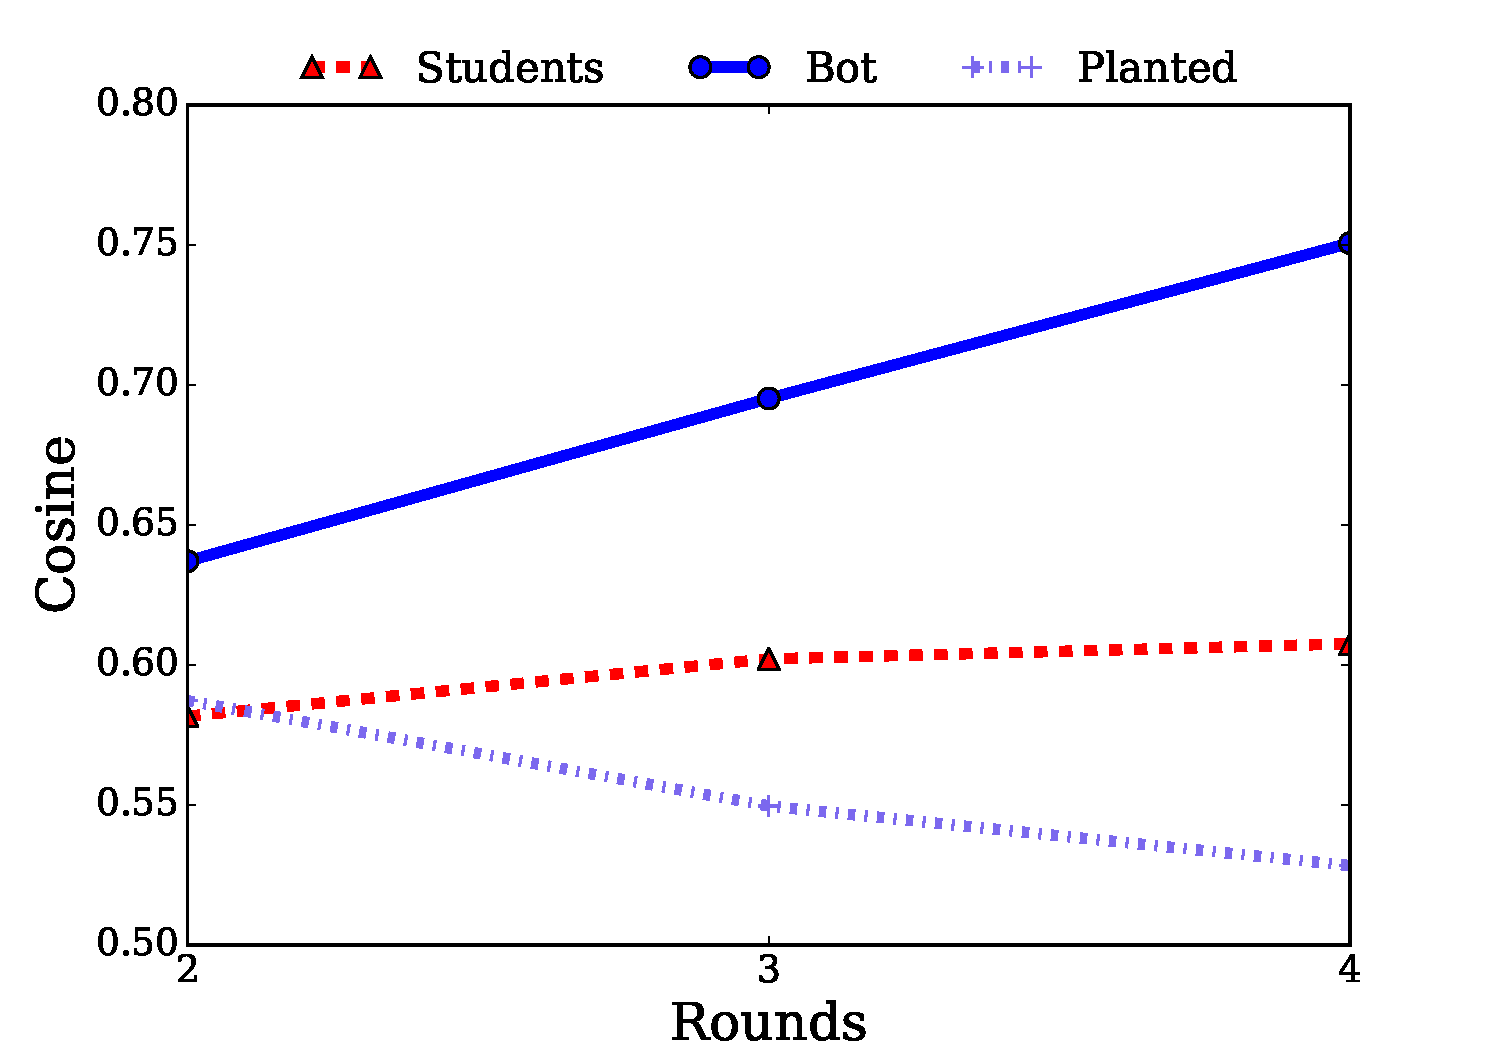
\includegraphics[width=8cm, height=5.5cm]{Results/similarity_to_winner} 
%\caption{\label{fig:simWinner} Similarity to the highest ranked document from the previous round.}
%\end{figure}

\begin{table}[t]
  \tabcolsep=0.2cm
  \caption{\label{tab:offHarmonic} Offline evaluation of the passage-pair ranking
    function with respect to the \random baseline;
    $\beta$ is used for both training and evaluation in the harmonic
    mean of the coherence and rank-promotion labels.
    %Note: each value of $\beta$ entails a
    %completely different experimental setting and hence the values of
    %all measures, except for TOP, are not comparable.
    `*' 
    marks statistically significant difference with 
    \random.}
  
  \begin{tabular}{@{}lcccccc@{}}
  \toprule
    & $\beta$ & MAP & NDCG@1 & NDCG@5 & P@1 & TOP \\ \midrule
%  \multicolumn{7}{|c|}{\harm} \\ \hline
%METHOD & $ \beta $ & MAP & NDCG_CUT.1 & NDCG_CUT.5 & P.1 & TOP1\\
%\hline
RankSVM & $0.0$ & $0.38^*$ & $0.22\;$ & $0.25^*$ & $0.37\;$ & $1.18\;$\\
Random & $0.0$ & $0.30\;$ & $0.14\;$ & $0.18\;$ & $0.26\;$ & $0.86\;$\\ \midrule
RankSVM & $0.5$ & $0.38^*$ & $0.23\;$ & $0.28^*$ & $0.33\;$ & $1.16\;$\\
Random & $0.5$ & $0.30\;$ & $0.16\;$ & $0.20\;$ & $0.26\;$ & $0.86\;$\\ \midrule
RankSVM & $1.0$ & $0.40^*$ & $0.22\;$ & $0.29^*$ & $0.33\;$ & $1.04\;$\\
Random & $1.0$ & $0.32\;$ & $0.18\;$ & $0.20\;$ & $0.28\;$ & $0.86\;$\\ \midrule
RankSVM & $2.0$ & $0.41^*$ & $0.30^*$ & $0.32^*$ & $0.44^*$ & $1.26^*$\\
Random & $2.0$ & $0.32\;$ & $0.21\;$ & $0.22\;$ & $0.29\;$ & $0.86\;$\\ \midrule
RankSVM & $10^3$ & $0.41^*$ & $0.32\;$ & $0.33^*$ & $0.42^*$ & $1.21\;$\\
Random & $10^3$ & $0.32\;$ & $0.23\;$ & $0.24\;$ & $0.29\;$ & $0.86\;$\\ \midrule
RankSVM & $10^5$ & $0.41^*$ & $0.32\;$ & $0.33^*$ & $0.42^*$ & $1.21\;$\\
Random & $10^5$ & $0.32\;$ & $0.23\;$ & $0.24\;$ & $0.29\;$ & $0.86\;$\\ \midrule
RankSVM & $10^9$ & $0.42^*$ & $0.36^*$ & $0.35^*$ & $0.46^*$ & $1.35^*$\\
Random & $10^9$ & $0.33\;$ & $0.22\;$ & $0.24\;$ & $0.30\;$ & $0.86\;$\\
\bottomrule
\end{tabular}

  %\begin{tabular}{@{}lcccccc@{}}
  \toprule
    & $\beta$ & MAP & NDCG@1 & NDCG@5 & P@1 & TOP \\ \midrule
%  \multicolumn{7}{|c|}{\harm} \\ \hline
%METHOD & $ \beta $ & MAP & NDCG_CUT.1 & NDCG_CUT.5 & P.1 & TOP1\\
%\hline
RankSVM & $0.0$ & $0.38^*$ & $0.22\;$ & $0.25^*$ & $0.37\;$ & $1.18\;$\\
Random & $0.0$ & $0.30\;$ & $0.14\;$ & $0.18\;$ & $0.26\;$ & $0.86\;$\\ \midrule
%RankSVM & $0.5$ & $0.38^*$ & $0.23\;$ & $0.28^*$ & $0.33\;$ & $1.16\;$\\
%Random & $0.5$ & $0.30\;$ & $0.16\;$ & $0.20\;$ & $0.26\;$ & $0.86\;$\\ \midrule
RankSVM & $1.0$ & $0.40^*$ & $0.22\;$ & $0.29^*$ & $0.33\;$ & $1.04\;$\\
Random & $1.0$ & $0.32\;$ & $0.18\;$ & $0.20\;$ & $0.28\;$ & $0.86\;$\\ \midrule
RankSVM & $2.0$ & $0.41^*$ & $0.30^*$ & $0.32^*$ & $0.44^*$ & $1.26^*$\\
Random & $2.0$ & $0.32\;$ & $0.21\;$ & $0.22\;$ & $0.29\;$ & $0.86\;$\\ \midrule
%RankSVM & $10^3$ & $0.41^*$ & $0.32\;$ & $0.33^*$ & $0.42^*$ & $1.21\;$\\
%Random & $10^3$ & $0.32\;$ & $0.23\;$ & $0.24\;$ & $0.29\;$ & $0.86\;$\\ \midrule
RankSVM & $10^5$ & $0.41^*$ & $0.32\;$ & $0.33^*$ & $0.42^*$ & $1.21\;$\\
Random & $10^5$ & $0.32\;$ & $0.23\;$ & $0.24\;$ & $0.29\;$ & $0.86\;$\\ 
%RankSVM & $10^9$ & $0.42^*$ & $0.36^*$ & $0.35^*$ & $0.46^*$ & $1.35^*$\\
%Random & $10^9$ & $0.33\;$ & $0.22\;$ & $0.24\;$ & $0.30\;$ & $0.86\;$\\
\bottomrule
\end{tabular}

\end{table}

\subsection{Results of the Offline Evaluation}
\label{sec:offlineResults}
%We now turn to describe the results of the offline evaluation of our
%RankSVM approach for ranking passage pair. (Refer back to Sect.
%\ref{sec:offline} for details regarding this offline evaluation
%setting.)
Table \ref{tab:offHarmonic} presents the offline evaluation of our
passage-pair ranking model.
Due to changes of labels, the performance numbers are not comparable across different values of $\beta$ except for TOP: the average rank promotion as a result of using the top passage-pair for document modification.

We can see in Table \ref{tab:offHarmonic}  that our approach outperforms the \random baseline for all
evaluation measures and all settings of $\beta$ --- the parameter that
governs the harmonic mean of the coherence and rank-promotion
labels. Most of the improvements are statistically significant.
In general, higher $\beta$, which means more weight put on rank promotion than on coherence for both training and evaluation, results in increased TOP values. 
Low values of $\beta$, result in 
 less statistically significant improvements in
terms of NDCG@1, P@1 and Top over the \random baseline. We also note
that the relatively effective performance of the \random baseline, specifically in terms of TOP, is
not surprising: this baseline, as our approach, replaces a passage in
a document with a passage from a document more highly ranked for the
query. Hence, there are decent chances, as the TOP values attest, that the replacement will result in rank promotion.

%\subsubsection{Alternative label integration}
%We followed work on integrating relevance and freshness labels for Web search \cite{Dai+al:11a} and integrated rank-promotion $r$ and coherence labels $c$ for passage pairs using the harmonic mean to yield labels $l$. In Table \ref{tab:offDemotex} we present the performance of our passage-pair ranking approach, with respect to the \random baseline, when using for both training and evaluation a ``label demotion'' approach inspired by that proposed in \citet{Dong+al:10a}. Specifically, if $0 \le \coherenceLabel < 2$, then $l \definedas \max \set{0,\rankPromoteLabel-2}$; if $2 \le \coherenceLabel < 4$, then $l \definedas \max \set{0,\rankPromoteLabel-1}$; if $ \coherenceLabel =4 $ then $l \definedas \rankPromoteLabel$. That is, the lower the coherence, the more penalty we impose on the rank-promotion label.

%We see in Table \ref{tab:offDemotex} that the improvements over the \random baseline are not statistically significant in almost all cases, and that the TOP numbers of our approach are much lower than those reported for the harmonic mean in Table \ref{tab:offHarmonic}. This findings attest to the merits of using the harmonic mean for label integration in our approach.


%\begin{table}[t]
%  \caption{\label{tab:offDemotex} Using a ``label demotion'' approach (cf. \protect\cite{Dong+al:10a}) to integrate rank-promotion and coherence labels for both training and evaluation. `*' marks a statistically significant difference with the \random baseline.}
%  \small
%  \begin{tabular}{@{}lccccc@{}}
  \toprule
    & MAP & NDCG@1 & NDCG@5 & P@1 & TOP \\ \midrule
RankSVM & $0.33^{*}$ & $0.16$ & $0.24$ & $0.25$ & $0.96$\\ 
Random & $0.26\:\:$ & $0.15$ & $0.18$ & $0.21$ & $0.86$ \\
\bottomrule
\end{tabular}

%\end{table}

\subsubsection{Feature Analysis}
Table \ref{tab:features} presents the feature weights, averaged over
the train folds, learned by the RankSVM passage-pair ranker. Feature weights are comparable as feature values are min-max
normalized.

We see that the weight of the \qryTermTarget feature,
which is a measure of query-terms occurrences in the passage to be
used for replacement, is the highest. Indeed, using passages that
contain many occurrences of query terms can help to improve retrieval
score, and hence ranking. The next two features with the highest
weights are \simTargetTopTF and \simTargetPrevTopWtV which are
measures of the similarity of a candidate replacing passage to the
documents most highly ranked in the current (\simTargetTopTF) and
previous (\simTargetPrevTopWtV) rankings. This finding provides
further support to the merits of mimicking documents most highly
ranked in the past for a given query. The next feature in terms of
weight is \simSrcPrevWtV which is the Word2Vec-based similarity of the
candidate replacing passage with the passage preceding the passage
which is a candidate to be replaced. This feature targets coherence
via semantic similarities with the context of the latter passage. Along the same lines, semantic
similarity of the candidate replacing passage to the passage following the candidate passage
to be replaced (\simTargetNextWtV) is assigned with the sixth highest
weight.


\begin{table}[t]
  \caption{\label{tab:features} Average feature weights, over the train folds, of our RankSVM approach for ranking passage pairs.}

  \center
  \begin{tabular}{@{}lc@{}}
\toprule
Feature & Weight \\
\midrule
QueryTermTarget & $\;\:\:0.590$ \\ 
SimTargetTop(T) & $\;\:\:0.262$ \\ 
SimTargetPrevTop(W) & $\;\:\:0.237$ \\
SimSrcPrecPsg(W) & $\;\:\:0.162$ \\ SimTargetPrevTop(T) & $\;\:\:0.147$ \\ 
SimTargetFollowPsg(W) & $\;\:\:0.139$ \\ 
SimTargetTop(W) & $\;\:\:0.120$ \\ 
SimSrcTop(W) & $\;\:\:0.070$ \\ 
SimSrcPrevTop(T) & $\;\:\:0.040$ \\ 
SimSrcTop(T) & $\;\:\:0.008$ \\ 
SimTargetPrecPsg(W) & $-0.046$ \\ 
SimSrcFollowPsg(W) & $-0.077$ \\ 
SimSrcPrevTop(W) & $-0.116$ \\ 
SimSrcTarget(W) & $-0.135$ \\ 
QryTermSrc & $-0.214$ \\ 
\bottomrule
\end{tabular}

\end{table}








